\documentclass[letterpaper,10pt]{memoir}

% 	\usepackage{amsmath,amsfonts,amssymb}

\usepackage{booktabs}

\usepackage{enumitem}

\usepackage[
	top=1in,
	inner=1in,
	outer=2.5in,
	bottom=1in,
	headsep=.35in,
	marginparwidth=1.25in,
	marginparsep=0.375in,
	]{geometry}

\usepackage{fancyhdr}
\pagestyle{fancy}
\fancyhead{}
\fancyfoot{}
\fancyhead[LE,RO]{\thepart \chaptermark\ page \thepage}
% \fancyhead[RE,LO]{\sectionmark \thepage}
% \fancyfoot[C]{\chaptername}

% 	\fancyhead[L]{**Left Header for all pages**}
% 	\fancyhead[R]{**Right Header for all pages**}


\usepackage{fourier-orns}
\renewcommand\headrule{{\color[rgb]{.75,.75,.75}\hrulefill
\raisebox{-2.1pt}[8pt][8pt]{\quad\decofourleft\decotwo\decofourright\quad}\hrulefill}}

% \renewcommand\headrule{
% \pgfornament[color=black!20,height=5mm]{88}}



\usepackage{graphicx}

\usepackage{lipsum}

\usepackage{hyperref}
\hypersetup{
	colorlinks=true,
	linkcolor=blue,
	urlcolor=blue,
}
	

\usepackage{listings}
\lstset{%
	basicstyle=\small,
	tabsize=3,
}

\usepackage{marginnote}

\usepackage{multicol}
\raggedcolumns

% \usepackage[percent]{overpic}

%%	TESTING
% \usepackage{pgfornament}

\usepackage{pstricks}

\usepackage{qrcode}

\usepackage{siunitx}

\usepackage[absolute]{textpos}
\textblockorigin{0in}{0in}


%%	Documentation encourages this package to be loaded last since
%%	it redefines many LaTeX commands. It is not clear how this package
%%	interacts with those above.
% \usepackage[hidelinks]{hyperref}

\usepackage{fourier} % or what ever
\usepackage[scaled=.92]{helvet}%. Sans serif - Helvetica
\usepackage{color,calc}
\newsavebox{\ChpNumBox}
\definecolor{ChapBlue}{rgb}{0.75,0.85,0.75}
\makeatletter
\newcommand*{\thickhrulefill}{%
\leavevmode\leaders\hrule height 1\p@ \hfill \kern \z@}

\newcommand*\BuildChpNum[2]{%
\begin{tabular}[t]{@{}c@{}}
\makebox[0pt][c]{#1\strut} \\[.5ex]
\colorbox{ChapBlue}{%
\rule[-10em]{0pt}{0pt}%
\rule{3ex}{0pt}\color{black}#2\strut
\rule{1ex}{0pt}}%
\end{tabular}}

\makechapterstyle{BlueBox}{%
\renewcommand{\chapnamefont}{\large\scshape}
\renewcommand{\chapnumfont}{\Huge\bfseries}
\renewcommand{\chaptitlefont}{\raggedright\Huge\bfseries}
\setlength{\beforechapskip}{20pt}
\setlength{\midchapskip}{26pt}
\setlength{\afterchapskip}{40pt}
\renewcommand{\printchaptername}{}
\renewcommand{\chapternamenum}{}
\renewcommand{\printchapternum}{%
\sbox{\ChpNumBox}{%
\BuildChpNum{\chapnamefont\@chapapp}%
{\chapnumfont\thechapter}}}
\renewcommand{\printchapternonum}{%
\sbox{\ChpNumBox}{%
\BuildChpNum{\chapnamefont\vphantom{\@chapapp}}%
{\chapnumfont\hphantom{\thechapter}}}}
\renewcommand{\afterchapternum}{}
\renewcommand{\printchaptertitle}[1]{%
\usebox{\ChpNumBox}\hfill
\parbox[t]{\hsize-\wd\ChpNumBox-2em}{%
\vspace{\midchapskip}%
% \thickhrulefill\par
\headrule\\[1mm]\par
\chaptitlefont ##1\par}}%
}
\chapterstyle{BlueBox}


	\newcommand{\filelister}[1]{%
		\lstinputlisting[language=Java, basicstyle=\footnotesize, numbers=left, numberstyle=\tiny, stepnumber=1, numbersep=5pt, xleftmargin=12pt]{../#1}
	}
	
	% \tiny 	sample text
	% \scriptsize 	sample text
	% \footnotesize 	sample text
	% \small 	sample text
	% \normalsize 	sample text
	
\usepackage{amsmath,amsfonts,amssymb}

\usepackage{booktabs}

\usepackage{enumitem}

\usepackage[
	top=1in,
	inner=1in,
	outer=1in,
	bottom=1in,
	headsep=.35in,
	marginparwidth=1.25in,
	marginparsep=0.375in,
	]{geometry}

\usepackage{fancyhdr}
\pagestyle{fancy}
\fancyhead{}
\fancyfoot{}
\fancyhead[LE,RO]{\thepart \chaptermark\ page \thepage}
% \fancyhead[RE,LO]{\sectionmark \thepage}
% \fancyfoot[C]{\chaptername}

% 	\fancyhead[L]{**Left Header for all pages**}
% 	\fancyhead[R]{**Right Header for all pages**}

	\usepackage{graphicx}
	
	\usepackage{listings}
	\lstset{%
		basicstyle=\small,
		tabsize=3,
	}

	\usepackage{siunitx}


%%
%%	DOCUMENT
%%
\begin{document}

% \tableofcontents

% \chapter{Software Configuration}

Programming and running the Onabots Robot requires six components. Each of these components requires the installation of software and configuration. Wherever possible, free open-source software is used.

\begin{enumerate}[label=$\Box$]

	\item Coding Computer. The Onabots use multiple computers running Debian GNU/Linux. Additional software includes OpenJDK 8, Eclipse with WPI plugins, Git, and ssh client.

	\item Driver Station. A Windows computer is required to control the robot as well as configure the OpenMesh Radio and the RoboRIO.

	\item OpenMesh Radio. The radio may be configured for wireless control at home but is reconfigured at tournaments to be restricted to the field wireless system.

	\item Raspberry PI. This computer runs the Raspian OS, a Debian OS for the Raspberry PI. The only other software this computer uses is Python3 with OpenCV for vision processing.

	\item RoboRIO. This requires two pieces of software to be installed: firmware and Java 8. If the firmware is updated, Java 8 will need to be reinstalled.

	\item Server. Computer running Debian GNU/Linux. Provides a web server and a version control system using git.
	
\end{enumerate}


	\subsection*{Networking}
	Check the FRC web site to ensure that these IP addresses do not conflict with the Field Management System, DHCP, or other addresses. Also confirm that the netmask are valid.
	\vspace*{3mm}

	{\renewcommand{\arraystretch}{1.5}
	\begin{tabular}{ @{} l l l p{3in} }
	\textbf{Component} & \textbf{Address} & \textbf{Netmask} & \textbf{Notes} \\
	\midrule
	OpenMesh Radio & 10.55.34.1 & n/a & Set automatically by radio configuration utility \\
	RoboRIO        & 10.55.34.2 & 255.255.255.0 \\
	DriverStation  & 10.55.34.5 & 255.0.0.0     & Note the different netmask for the driver station \\
	Raspberry PI   & 10.55.34.6 & 255.255.255.0 & Address does not matter unless not using networktables \\
	\end{tabular}
	}




\newpage\section*{Coding Computers}

\begin{itemize}
\item OpenJDK 8
\item Eclipse
\item Git
\end{itemize}


\section*{Driver Station}
\begin{itemize}
\item FRC 2018 Update Suite
\end{itemize}


\section*{OpenMesh Radio}
\begin{itemize}
\item Firmware
\item Configure
\end{itemize}


\section*{Raspberry PI}
\begin{itemize}
\item Raspian OS
\item Python3
\item Other stuff
\item OpenCV
\end{itemize}


\section*{RoboRIO}
\begin{itemize}
\item Firmware
\item Oracle Java
\end{itemize}


\section*{Server}
\begin{itemize}
\item apache2
\item git
\item ssh
\end{itemize}



Also recommend using a combination of Git server and GitHub for public code sharing.
%
I recommend keeping all documentation, vision code, and robot code in the same repository.



\newpage\section*{OpenMesh Radio}

\begin{itemize}
\item Label radio with team number and year with piece of masking tape. This is needed at tournaments when the field judges configure the radio. Keep a radio configured for home use so that it does not have to be reconfigured. This also allows us to use the robot wirelessly during practice. Indicate whether this is the tournament or home radio.

\item Configure the radio. This may need to be check later to see if there is a more up-to-date version. Note that `IL' represents a version used in Israel.

\item Radio is powered by the VRM 12V/2A port. Strip 5/16 inn from wires.

\item For power, the center of the barrel is positive. Red should be connected to the center. Black is for the outside.
\end{itemize}


\subsection*{Firmware}

Must be performed using a Windows computer.

\begin{enumerate}
\item Disable WiFi on Control Panel

\item Open FRC Radio Configuration Utility from desktop

\item Select Ethernet as network interface

\item Enter team number (e.g., 5534)

\item Make sure the radio is on OpenMesh

\item Press `Load Firmware'

\item Follow on-screen directions pertaining to power cycling

\item After the firmware is loaded, wait for about 2 minutes until the power light has stopped flashing for about a minute.

\item Press `Configure'

\item Done
\end{enumerate}



% \chapter{Calendar}
% 
% The schedule for robotics season is all-year. However, certain task have expected dates due to knowledge of the competition, tasks, etc.
% 
% Include references to other documents. Preferably hyper-links.




% \chapter{Components}
% 
% \begin{itemize}
% \item Motor Controller
% \item Encoder
% \item Range Finder
% \item Camera
% \item Power Distribution Panel
% \item RoboRIO
% \item Pneumatics Control Module
% \item Voltage Regulator Module
% \end{itemize}


%%
%% ROBORIO
%%
% \newpage\section*{RoboRIO}
% 
% Some information about the RoboRIO.
% 
% 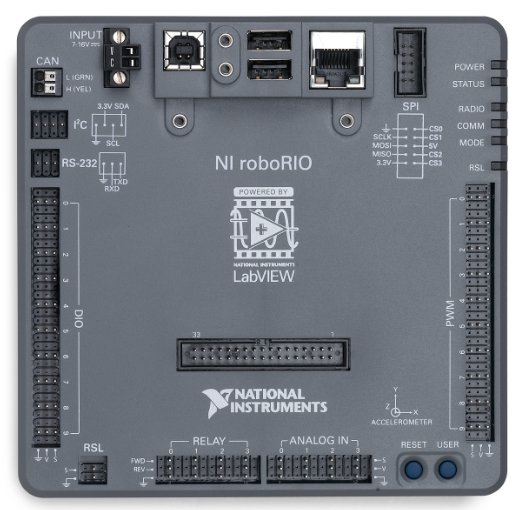
\includegraphics[width=\textwidth]{images/ni_roborio}
% 
% Include information about the various ports, their naming.
% 
% INPUT Power for RoboRIO. Do not use screws facing top, these hold the black plastic to the RoboRIO. Screws to tighten wires are found on the left side of the black plastic.
% 
% Another picture showing the labelled parts of the roborio would be good.


%%
%%	MOTOR CONTROLLERS
%%
% \newpage\section*{Motor Controllers}
% 
% 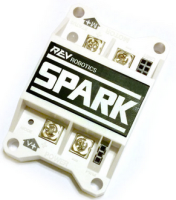
\includegraphics[width=.25\textwidth]{images/spark}
% 
% 
% \subsection*{Notes}
% \begin{itemize}
% \item Different types of motor controllers. Onabots use Sparks due to low price. Have not met any limitations.
% 
% \item A motor controller can control more than one motor but need a PWM split cable.
% 
% \item Talk about PWM, as Pulse Width Modulated. Varies the amount of time that a voltage is applied to the motor.
% 
% \item Range of motor controller values: \SIrange{-1}{1}{} with \num{0} denoting no power.
% 
% \item Actually good to set motor speed from an encoder instead of motor power. Speed changes with friction, frame resistance, and battery voltage.
% 
% \item Wiring requirements, what size gauge is needed?
% 
% \item Braking vs Coast mode (has not been used)
% 
% \item 
% \end{itemize}
% 
% \subsection*{Java}
% \lstset{language=Java}
% \begin{lstlisting}[language=Java]
% 	// DEFINE SPARK
% 	public static Spark DriveMotorRF = new Spark( Ports.PWM_DriveMotorRF );
% 
% 	// SET POWER
% 	DriveMotorRF.set( 0.50 );
% \end{lstlisting}
% 


%%
%%	RADIO
%%
% \newpage\section*{Radio}





%%
%%	ENCODERS
%%
% \newpage\section*{Encoders}
% 
% Encoders should be used anywhere you need to control motor speed.




% At the beginning of each of these files include the purpose and constraints for code that must exist there.
% 
% Include a program flow for each mode.

%%
%%
%%

% \chapter{Eclipse}


\section{Installation}

\begin{enumerate}
\item Install Java 8
\end{enumerate}



\section{Configuration}

% Plugins


\section{Creating a Project}

% Example project



Steps to follow. Include pictures and possibly links to video.

\begin{itemize}
	\item Download and Install Java 8 from Oracle web site
	\item Download and Install Ecilpse for following site
	\item Install WPI plugin
	\item Configure Eclipse
	\item Firmware in RoboRIO
	\item Configure access points
	\item Update firmware (see yellow paper, Not IS - that is for Israeli teams)
	\item Vision tracking set-up with RaspberryPI
\end{itemize}



%%
%%	ROBOT CODE
%%
\newpage\chapter{Robot Code}

%%
%%
%%
	\newpage\section*{Robot.java}
	\filelister{Robot.java}

	\newpage\section*{Onabot.java}
	\filelister{Mode/Onabot.java}

	\newpage\section*{Autonomous.java}
	\filelister{Mode/Autonomous.java}

% 	\newpage\section*{Disabled.java}
% 	\filelister{Mode/Disabled.java}

	\newpage\section*{Teleop.java}
	\filelister{Mode/Teleop.java}

%%
%%
%%
	\newpage\section*{Autopilot.java}
	
	The Autopilot methods are used in Autonomous mode to set the chassis speed variable found in this class. Values are sent to motor controllers in Autonomous.Periofic().
	
	\filelister{Hardware/Autopilot.java}

	\newpage\section*{Driver.java}
	\filelister{Hardware/Driver.java}

	\newpage\section*{Elevator.java}
	\filelister{Hardware/Elevator.java}

	\newpage\section*{ElevArm.java}
	\filelister{Hardware/ElevArm.java}

	\newpage\section*{ElevClaw.java}
	\filelister{Hardware/ElevClaw.java}

	\newpage\section*{ElevLift.java}
	\filelister{Hardware/ElevWrist.java}

	\newpage\section*{ElevWrist.java}
	\filelister{Hardware/ElevWrist.java}

	\newpage\section*{EncTalonFX.java}
	\filelister{Hardware/EncTalonFX.java}

	\newpage\section*{Module.java}
	\filelister{Hardware/Module.java}

	\newpage\section*{Navigation.java}
	\filelister{Hardware/Navigation.java}

	\newpage\section*{Settings.java}
	\filelister{Hardware/Settings.java}

	\newpage\section*{Stage.java}
	\filelister{Hardware/Stage.java}

	\newpage\section*{Swerve.java}
	\filelister{Hardware/Swerve.java}

	\newpage\section*{Track.java}
	\filelister{Hardware/Track.java}

	
	\newpage\section*{Default.java (Driver)}
	\filelister{Driver/Default.java}



% 
% 
% \newpage\chapter{Java Tutorial}
% 



\end{document}

